\section{Experimento 2: Resultados con variables transformadas}
\label{sec:resultados_features_transformadas}

La Sección~\ref{sec:resultados_features_original} presentó los resultados del $\Delta$AIC 
para las variables en escala original. En esta sección se evalúa el efecto 
de aplicar transformaciones sobre dichas variables, con el objetivo de 
determinar si una representación alternativa mejora su capacidad predictiva 
sobre la señal EEG. 

\subsection{Diagnóstico de multicolinealidad (VIF)}

Al igual que para las variables en escala original, se calculó el VIF 
para cada variable transformada incorporándola individualmente al modelo 
base MD2. La Tabla~\ref{tab:vif_features_transformadas} reporta la 
media, la mediana y el porcentaje de sujetos con VIF superior a 3 y 
a 5 para cada variable transformada.

\begin{table}[H]
\centering
\small
\resizebox{\textwidth}{!}{%
\begin{tabular}{lcccc}
\toprule
\textbf{Variable} & \textbf{Media} & \textbf{Mediana} & \textbf{\% sujetos VIF $>$ 3} & \textbf{\% sujetos VIF $>$ 5} \\
\midrule
\multicolumn{5}{l}{\textit{Bottom-up}} \\
\feat{saliencia\_pixel\_log}        & 2.83 & 2.78 & 11.9 & 0.0 \\
\feat{saliencia\_media\_log}        & 3.09 & 3.08 & 54.8 & 0.0 \\
\midrule
\multicolumn{5}{l}{\textit{Similitud con el target}} \\
\feat{similitud\_pixel\_log}        & 2.85 & 2.85 & 4.8  & 0.0 \\
\feat{similitud\_media\_log}        & 3.67 & 3.65 & 100.0 & 0.0 \\
\midrule
\multicolumn{5}{l}{\textit{Estado interno del proceso bayesiano}} \\
\feat{ganancia\_informacion\_log}   & 4.46 & 4.50 & 100.0 & 7.1 \\
\feat{posterior\_log}               & 10.50 & 10.47 & 100.0 & 100.0 \\
\feat{posterior\_logit}             & 9.88 & 9.91 & 100.0 & 100.0 \\
\midrule
\multicolumn{5}{l}{\textit{Calidad de la decisión}} \\
\feat{gap\_entropia\_log}           & 1.43 & 1.43 & 0.0  & 0.0 \\
\feat{distancia\_grilla\_log}       & 5.69 & 5.63 & 100.0 & 92.9 \\
\midrule
\multicolumn{5}{l}{\textit{Competencia entre candidatos}} \\
\feat{competencia\_densidad\_log}   & 6.36 & 6.49 & 100.0 & 100.0 \\
\feat{competencia\_fp\_max\_log}    & 1.48 & 1.48 & 0.0  & 0.0 \\
\bottomrule
\end{tabular}%
}
\caption{VIF calculado por sujeto para cada variable transformada,
incorporada individualmente al modelo base MD2. Se reportan la 
media y mediana grupal ($n = 42$) y el porcentaje de sujetos que 
superan los umbrales de VIF $>$ 3 y VIF $>$ 5.}
\label{tab:vif_features_transformadas}
\end{table}

Se puede observar en la tabla cómo algunas de las transformaciones introducen multicolinealidad problemática 
con los predictores del modelo base. Las transformaciones 
\feat{posterior\_log} y \feat{posterior\_logit} presentaron los 
valores más elevados, con medias de 10.50 y 9.88 respectivamente 
y el 100\% de los sujetos superando el umbral de VIF $> 5$. 
\feat{competencia\_densidad\_log} y \feat{distancia\_grilla\_log} 
también superaron dicho umbral, con medias de 6.36 y 5.69 y el 
100\% y 92.9\% de los sujetos afectados respectivamente. Estas 
cuatro variables fueron descartadas del análisis de $\Delta$AIC 
y TFCE correspondiente.

Las 7 variables transformadas restantes presentaron valores de VIF 
aceptables.


\subsection{Evaluación individual de variables mediante $\Delta$ AIC}

Para cada variable, se compara el $\Delta$AIC obtenido 
al incorporar la versión transformada al modelo base MD2 contra el 
$\Delta$AIC correspondiente a la versión en escala original. En la mayoría de los casos la transformación 
$\log(x)$ mejora el ajuste respecto a la versión base, con la 
excepción de \feat{gap\_entropia\_log}.

\begin{figure}[H]
    \centering
    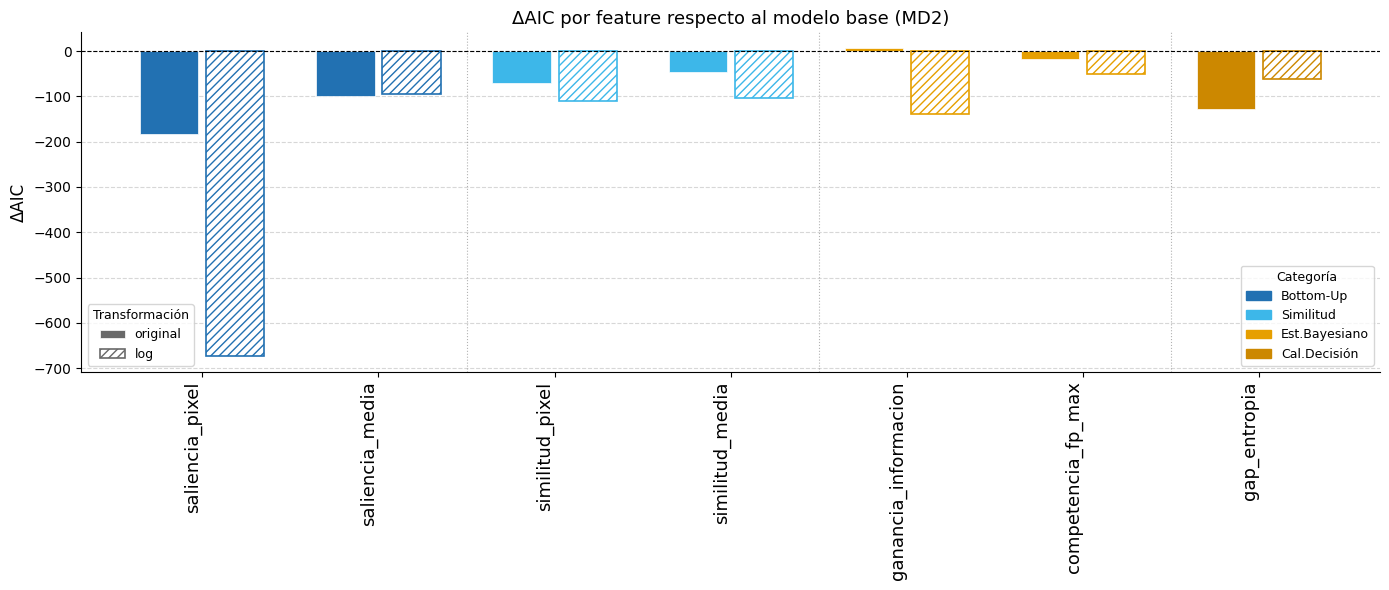
\includegraphics[width=\textwidth]{chapters/05_resultados/images/delta_aic_transformadas}
    \caption{$\Delta$AIC para variables en escala original y transformadas, coloreadas por categoría}
    \label{fig:delta_aic_transformadas}
\end{figure}

\begin{sloppypar}

La variable \feat{saliencia\_pixel\_log} presenta 
la mayor ganancia de todo el conjunto evaluado, consolidándose 
como la variable con mayor capacidad predictiva sobre la señal EEG. 
En contraste, \feat{saliencia\_media\_log} no muestra una mejora 
apreciable respecto a su versión original, sugiriendo que la transformación logarítmica no 
aporta información adicional para esta variable.

En la categoría de similitud con el target, tanto 
\feat{similitud\_pixel\_log} como \feat{similitud\_media\_log} muestran mejoras moderadas respecto 
a sus versiones originales.

En el caso de \feat{ganancia\_informacion}, la transformación produce el cambio más pronunciado. Mientras que en escala original su $\Delta$AIC era positivo , la transformación 
$\log(x)$ revierte este comportamiento de forma marcada. Este resultado sugiere que la 
relación entre \feat{ganancia\_informacion} y la señal EEG es 
esencialmente no lineal en escala original, y que la transformación 
logarítmica captura esta relación de forma más adecuada.

En la categoría de competencia entre candidatos, 
\feat{competencia\_fp\_max\_log} muestra una mejora moderada 
respecto a su versión original.

Finalmente, \feat{gap\_entropia\_log} es el único caso en que 
la transformación empeora el ajuste respecto a la versión original, lo que indica que 
la escala original captura mejor la relación de esta variable con 
la señal EEG.

\end{sloppypar}

\subsection{Resultados TFCE}

Se aplicó el test TFCE 
para las 7 variables transformadas que superaron el diagnóstico de multicolinealidad.
Para cada variable, los resultados se comparan con 
los obtenidos en su versión en escala original, con el objetivo de 
determinar si la transformación modifica no solo la magnitud del 
$\Delta$AIC sino también la presencia y extensión de clusters 
espacio-temporales significativos. Los resultados se organizan en 
tres grupos: variables con clusters significativos en ambas versiones, 
variables que obtienen clusters significativos únicamente en la versión 
transformada, y variables sin clusters significativos en ninguna de las 
dos versiones.

\subsubsection{Variables con clusters significativos en ambas versiones}

Las variables \feat{saliencia\_pixel}, \feat{saliencia\_media} y 
\feat{similitud\_pixel} presentaron clusters significativos tanto en 
su versión en escala original como en su versión transformada, aunque 
con diferencias en la extensión espacio-temporal de los clusters.

La transformación logarítmica de \feat{saliencia\_pixel} conserva el efecto observado en escala original, aunque con diferencias en amplitud y extensión; en ambas versiones se identifica un efecto temprano con topografía occipital. La amplitud de la TRF es considerablemente menor en la versión logarítmica, lo que es esperable dado que la transformación comprime los valores extremos. Un hallazgo que se repite en ambas versiones es la presencia de activación significativa en el período previo al onset de la fijación.

\begin{figure}[H]
    \centering
    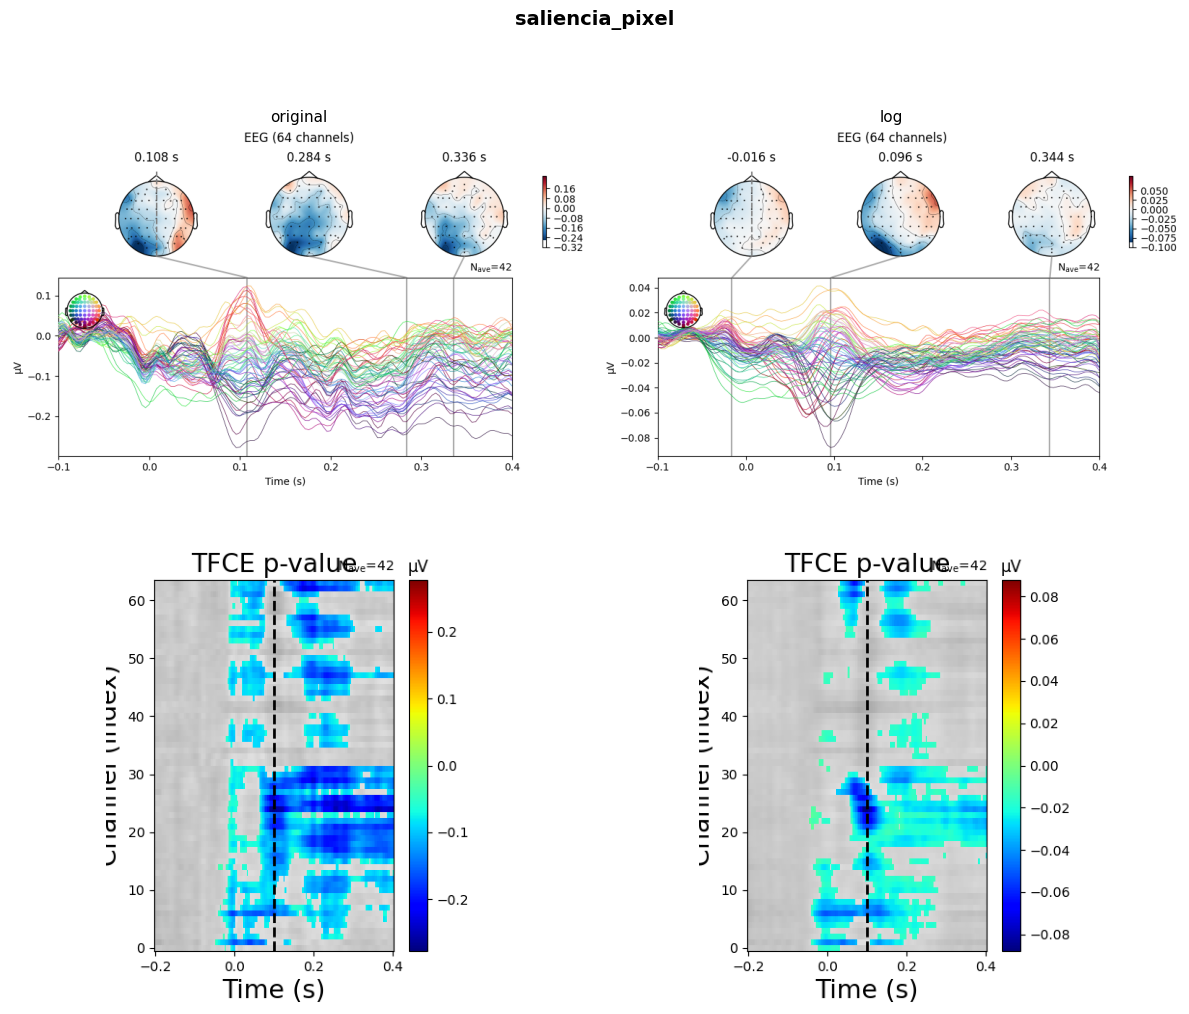
\includegraphics[width=0.7\textwidth]{chapters/05_resultados/images/TFCE_saliencia_pixel.png}
    \caption{Comparación resultados de TFCE para \feat{saliencia\_pixel} original y transformada en escala logarítmica.}
    \label{fig:tfce_saliencia_pixel}
\end{figure}

En los resultados de \feat{saliencia\_media} se puede observar cómo la señal de la versión logarítmica es más limpia que la señal de la escala original, aunque con menor amplitud. La topografía negativa occipital aparece más concetrada y localizada. Sin embargo, el cluster TFCE es considerablemente más pequeño y acotado que en la versión original. La activación pre-onset presente en la versión original no se observa en la versión logarítmica.

\begin{figure}[H]
    \centering
    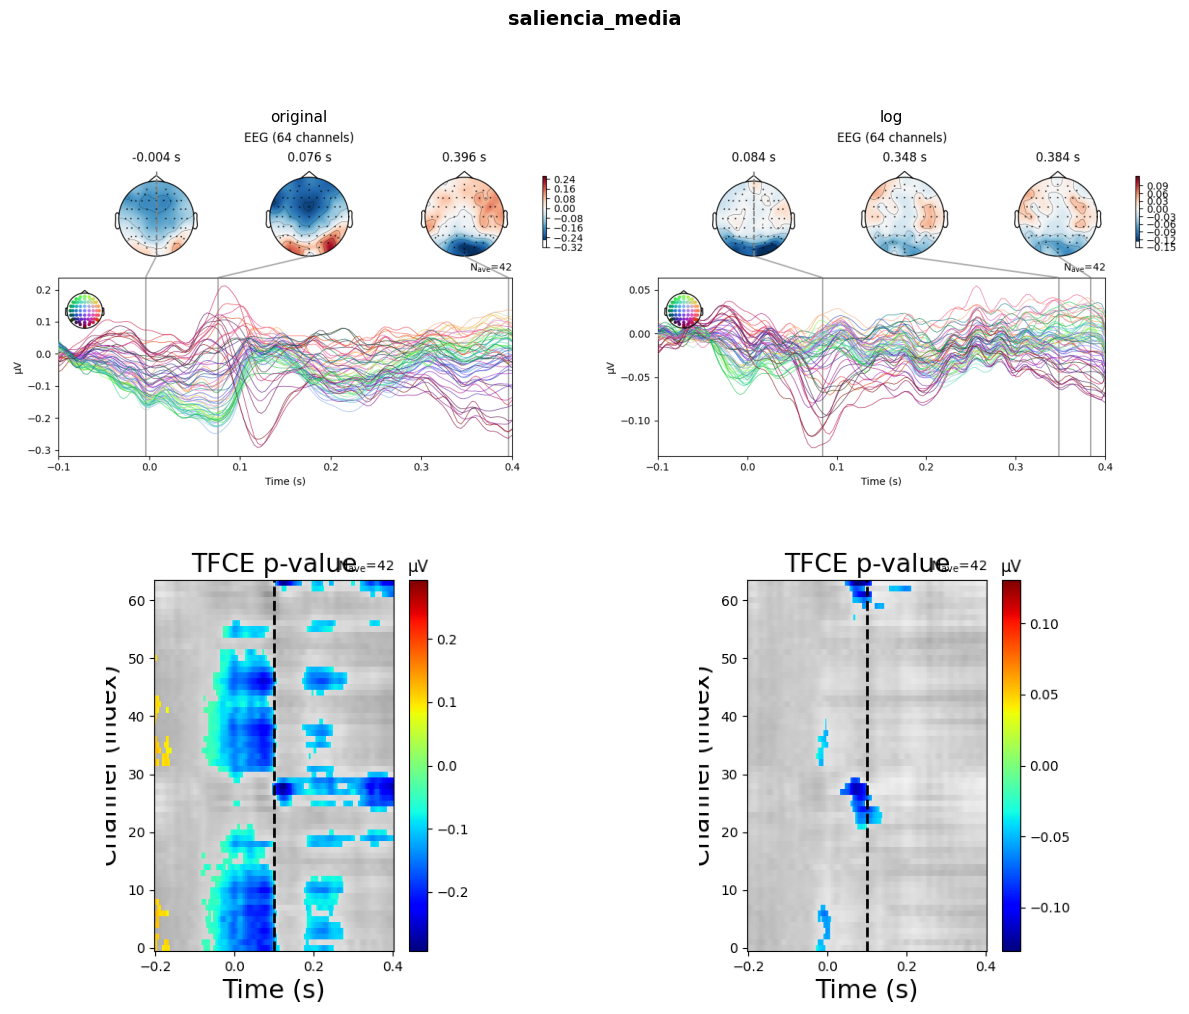
\includegraphics[width=0.7\textwidth]{chapters/05_resultados/images/TFCE_saliencia_media.png}
    \caption{Comparación resultados de TFCE para \feat{saliencia\_media} original y transformada en escala logarítmica.}
    \label{fig:tfce_saliencia_media}
\end{figure}

En su versión logarítmica \feat{similitud\_pixel} presenta una activación negativa más pronunciada que en escala original. La topografía a 80 ms es occipital, más limpia y localizada que en la versión original, donde el patrón era más difuso. El cluster TFCE resultante es también más concentrado espacialmente.

\begin{figure}[H]
    \centering
    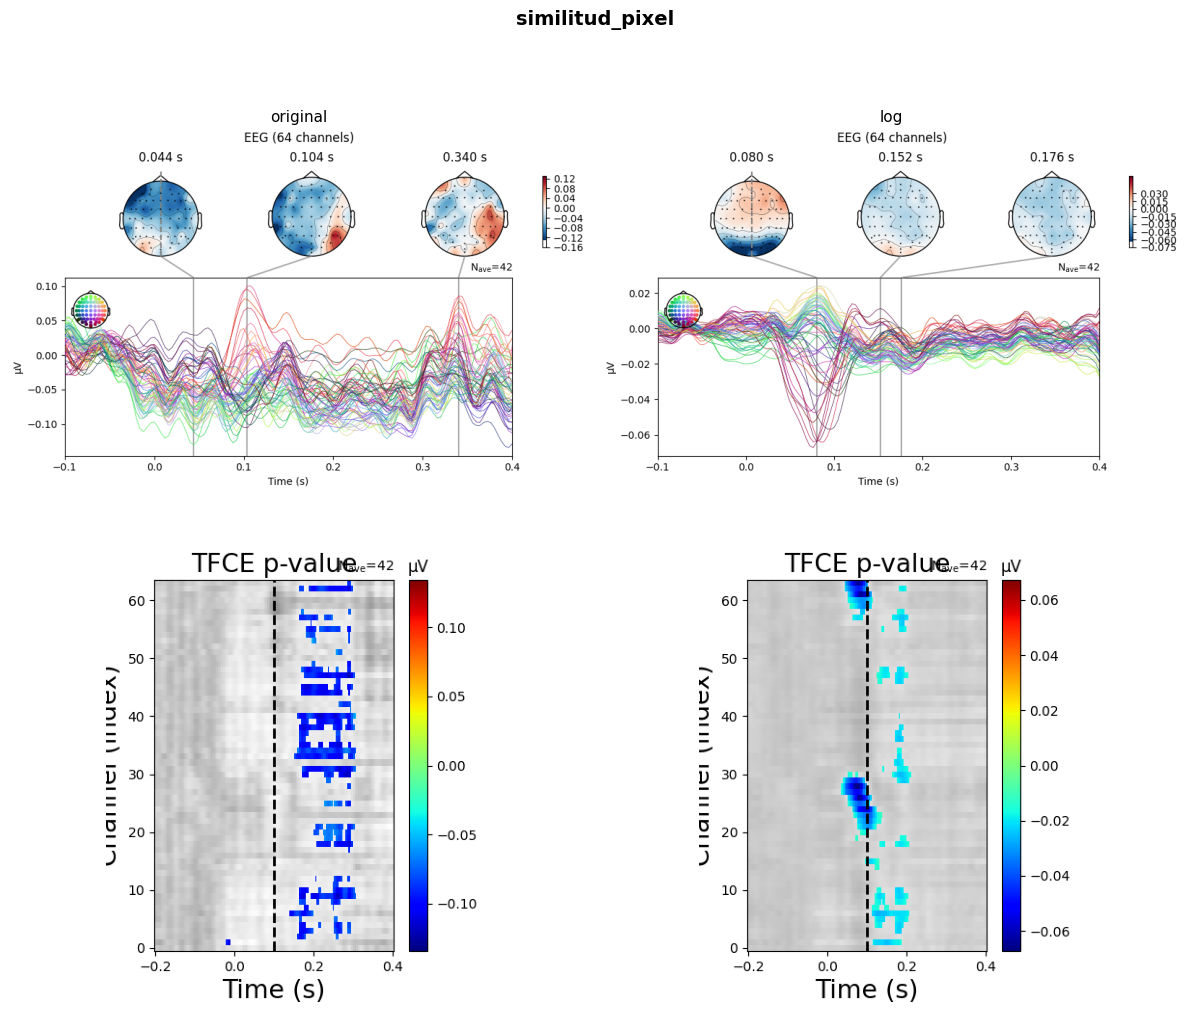
\includegraphics[width=0.7\textwidth]{chapters/05_resultados/images/TFCE_similitud_pixel.png}
    \caption{Comparación resultados de TFCE para \feat{similitud\_pixel} original y transformada en escala logarítmica.}
    \label{fig:tfce_similitud_pixel}
\end{figure}

\subsubsection{Variables con clusters significativos solo en la versión transformada}

Las variables \feat{similitud\_media}, \feat{ganancia\_informacion} y 
\feat{gap\_entropia} no presentaron clusters significativos en escala 
original pero sí en su versión transformada, lo que indica que la 
transformación logarítmica permite detectar efectos que no eran 
evidentes en la escala original.

Para \feat{similitud\_media} en escala original la señal es ruidosa y sin estructura, y el cluster TFCE es inexistente. En la versión logarítmica emerge una señal limpia con una activación positiva y una topografía fronto-central clara. La topografía fronto-central contrasta con el patrón occipital observado en \feat{similitud\_pixel}.

\begin{figure}[H]
    \centering
    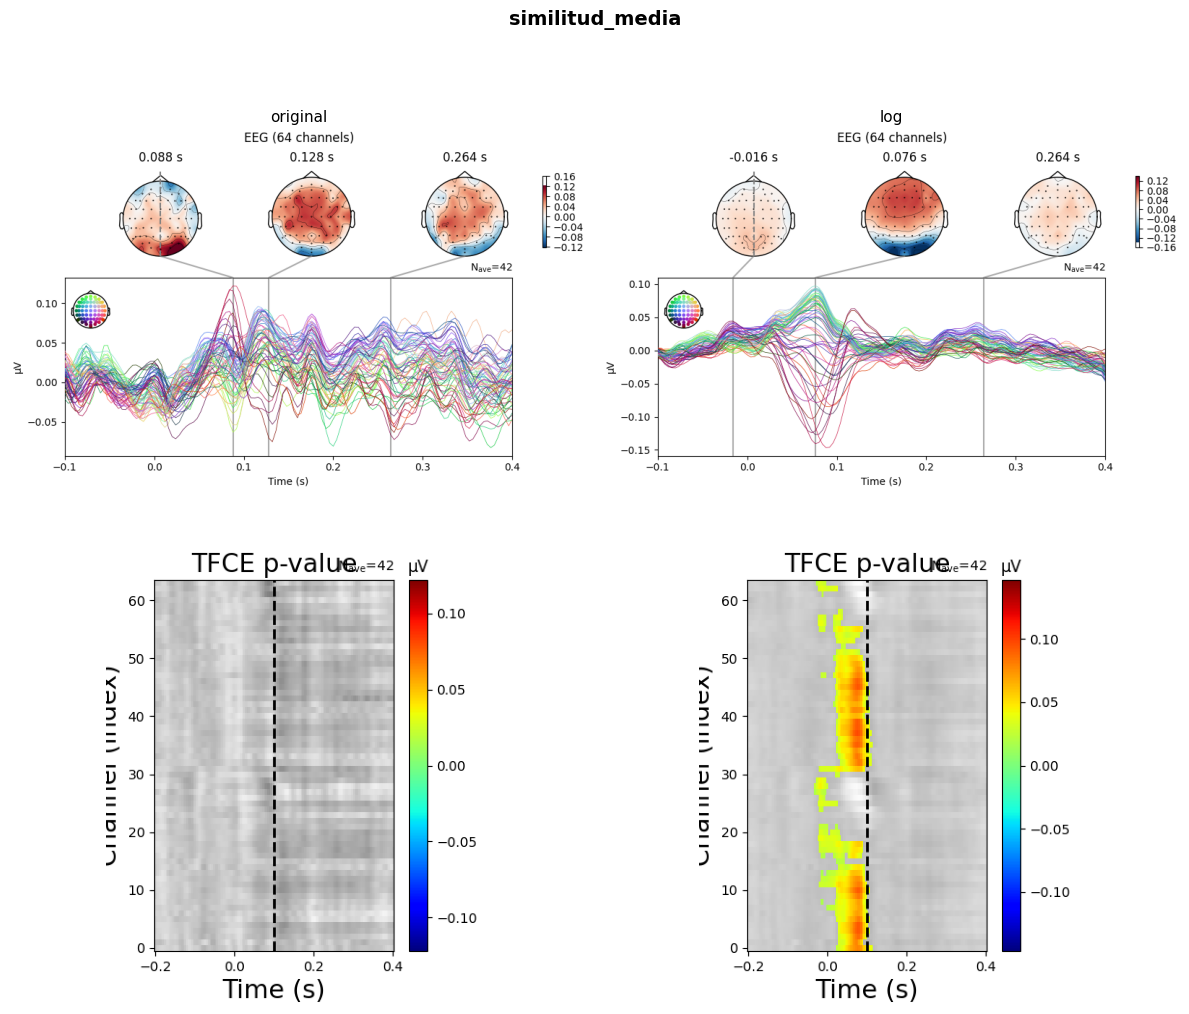
\includegraphics[width=0.7\textwidth]{chapters/05_resultados/images/TFCE_similitud_media.png}
    \caption{Comparación resultados de TFCE para \feat{similitud\_media} original y transformada en escala logarítmica.}
    \label{fig:tfce_similitud_media}
\end{figure}

En escala original \feat{ganancia\_informacion} no produce cluster significativos y su $\Delta$ AIC es el único positivo del conjunto. La versión logarítmica revierte este resultado: aparece una activación negativa con topografía de mayor intensidad en canales centrales y parietales.

\begin{figure}[H]
    \centering
    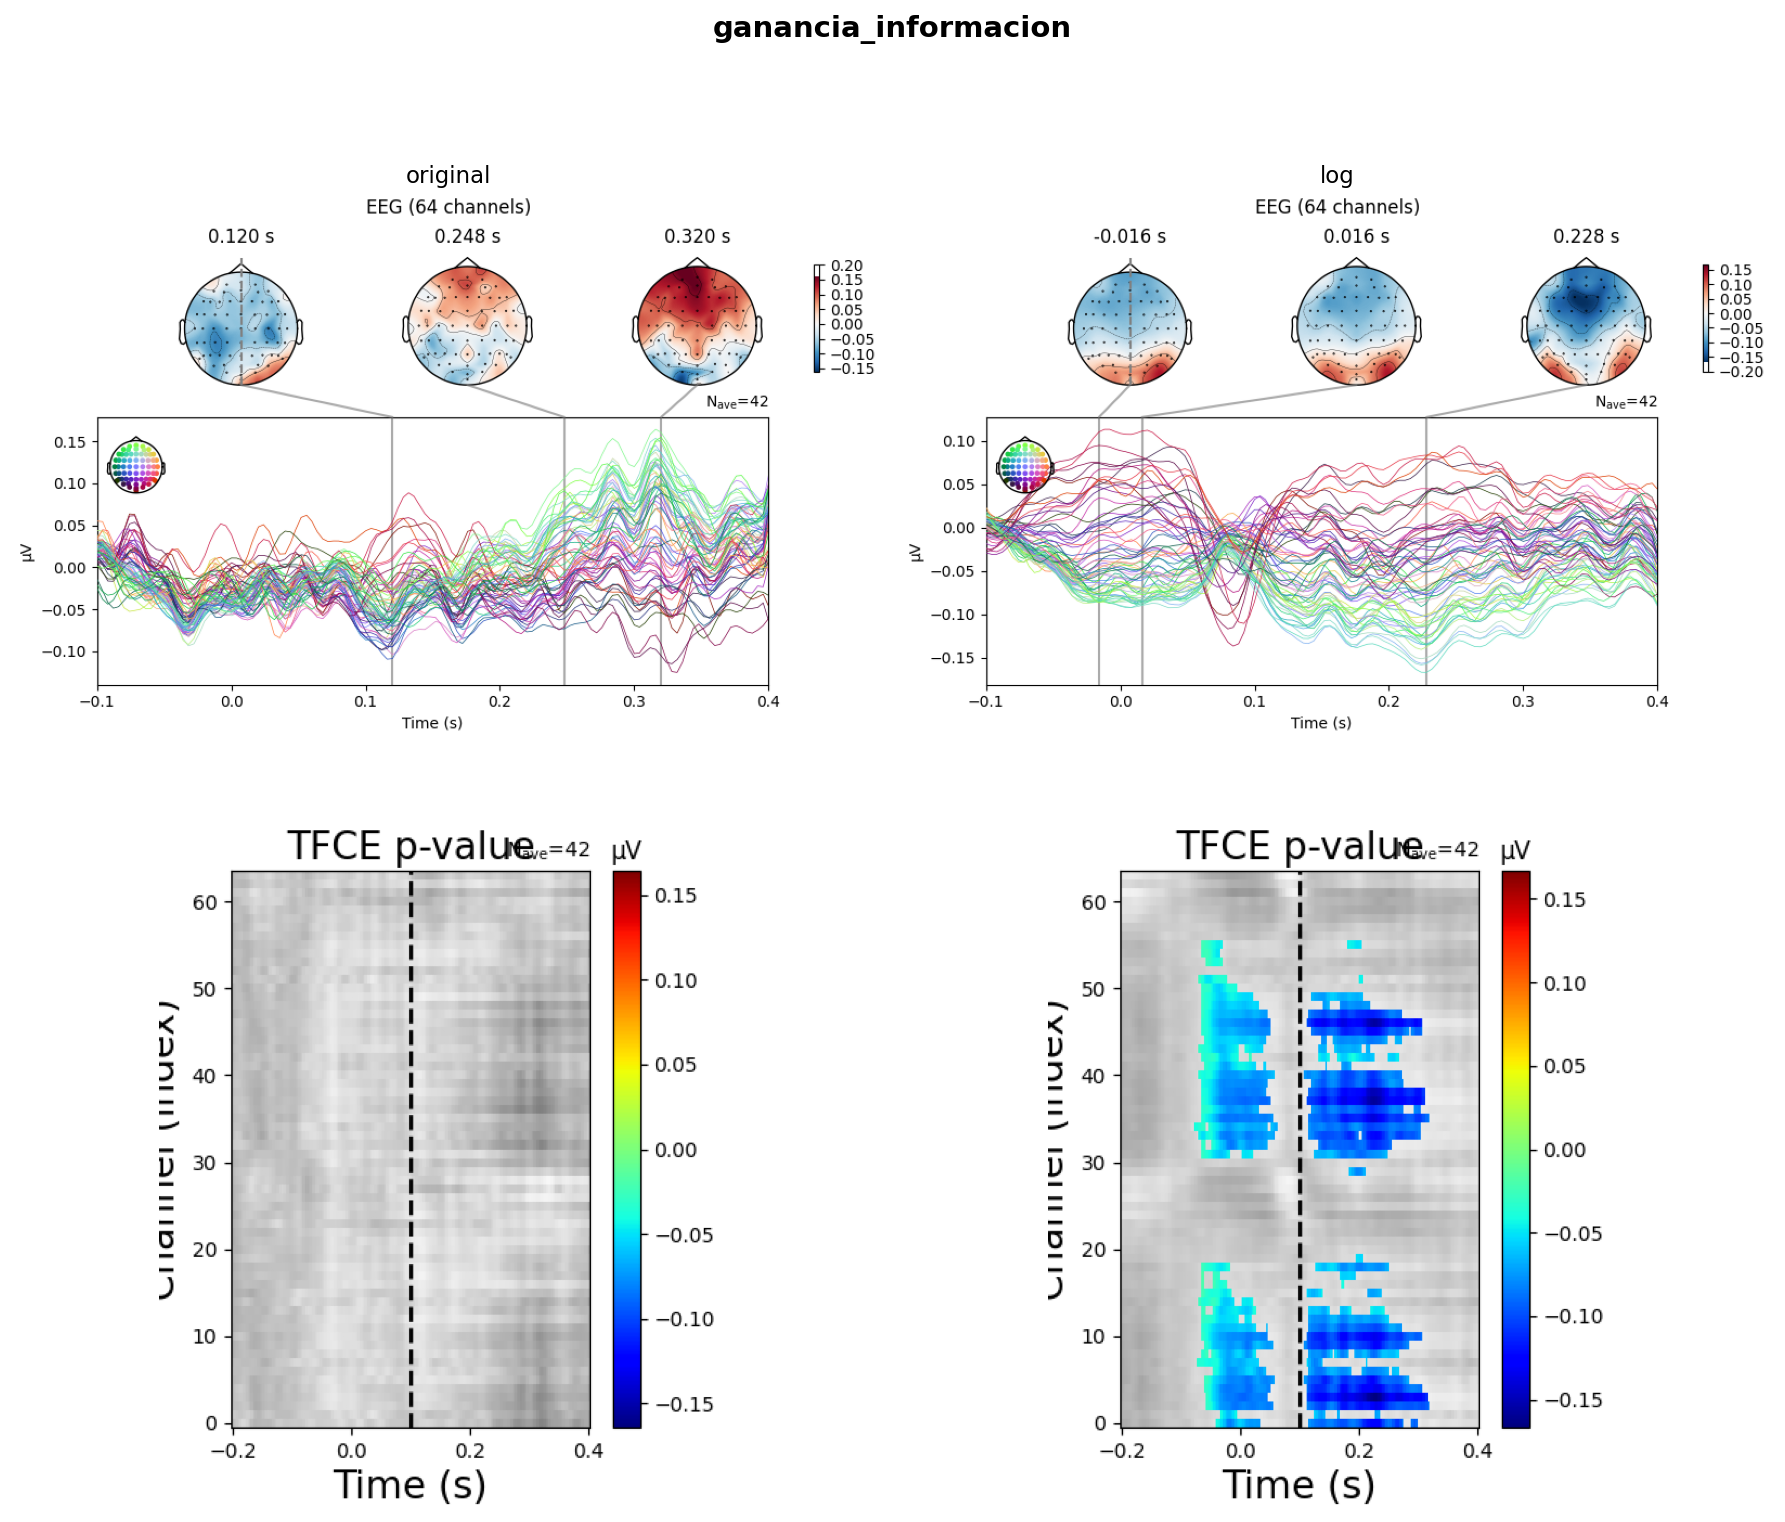
\includegraphics[width=0.7\textwidth]{chapters/05_resultados/images/TFCE_ganancia_informacion.png}
    \caption{Comparación resultados de TFCE para \feat{ganancia\_informacion} original y transformada en escala logarítmica.}
    \label{fig:tfce_ganancia_informacion}
\end{figure}

El cluster resultante de aplicar transformación logarítmica a \feat{ganancia\_informacion} es negativo y la distribución espacio-temporal observada es similar a la de \feat{ganancia\_informacion} en escala logarítmica. Como punto llamativo, la topografía observada a $\sim$80ms en la versión logarítmica es inversa a la observada en escala original. 

\begin{figure}[H]
    \centering
    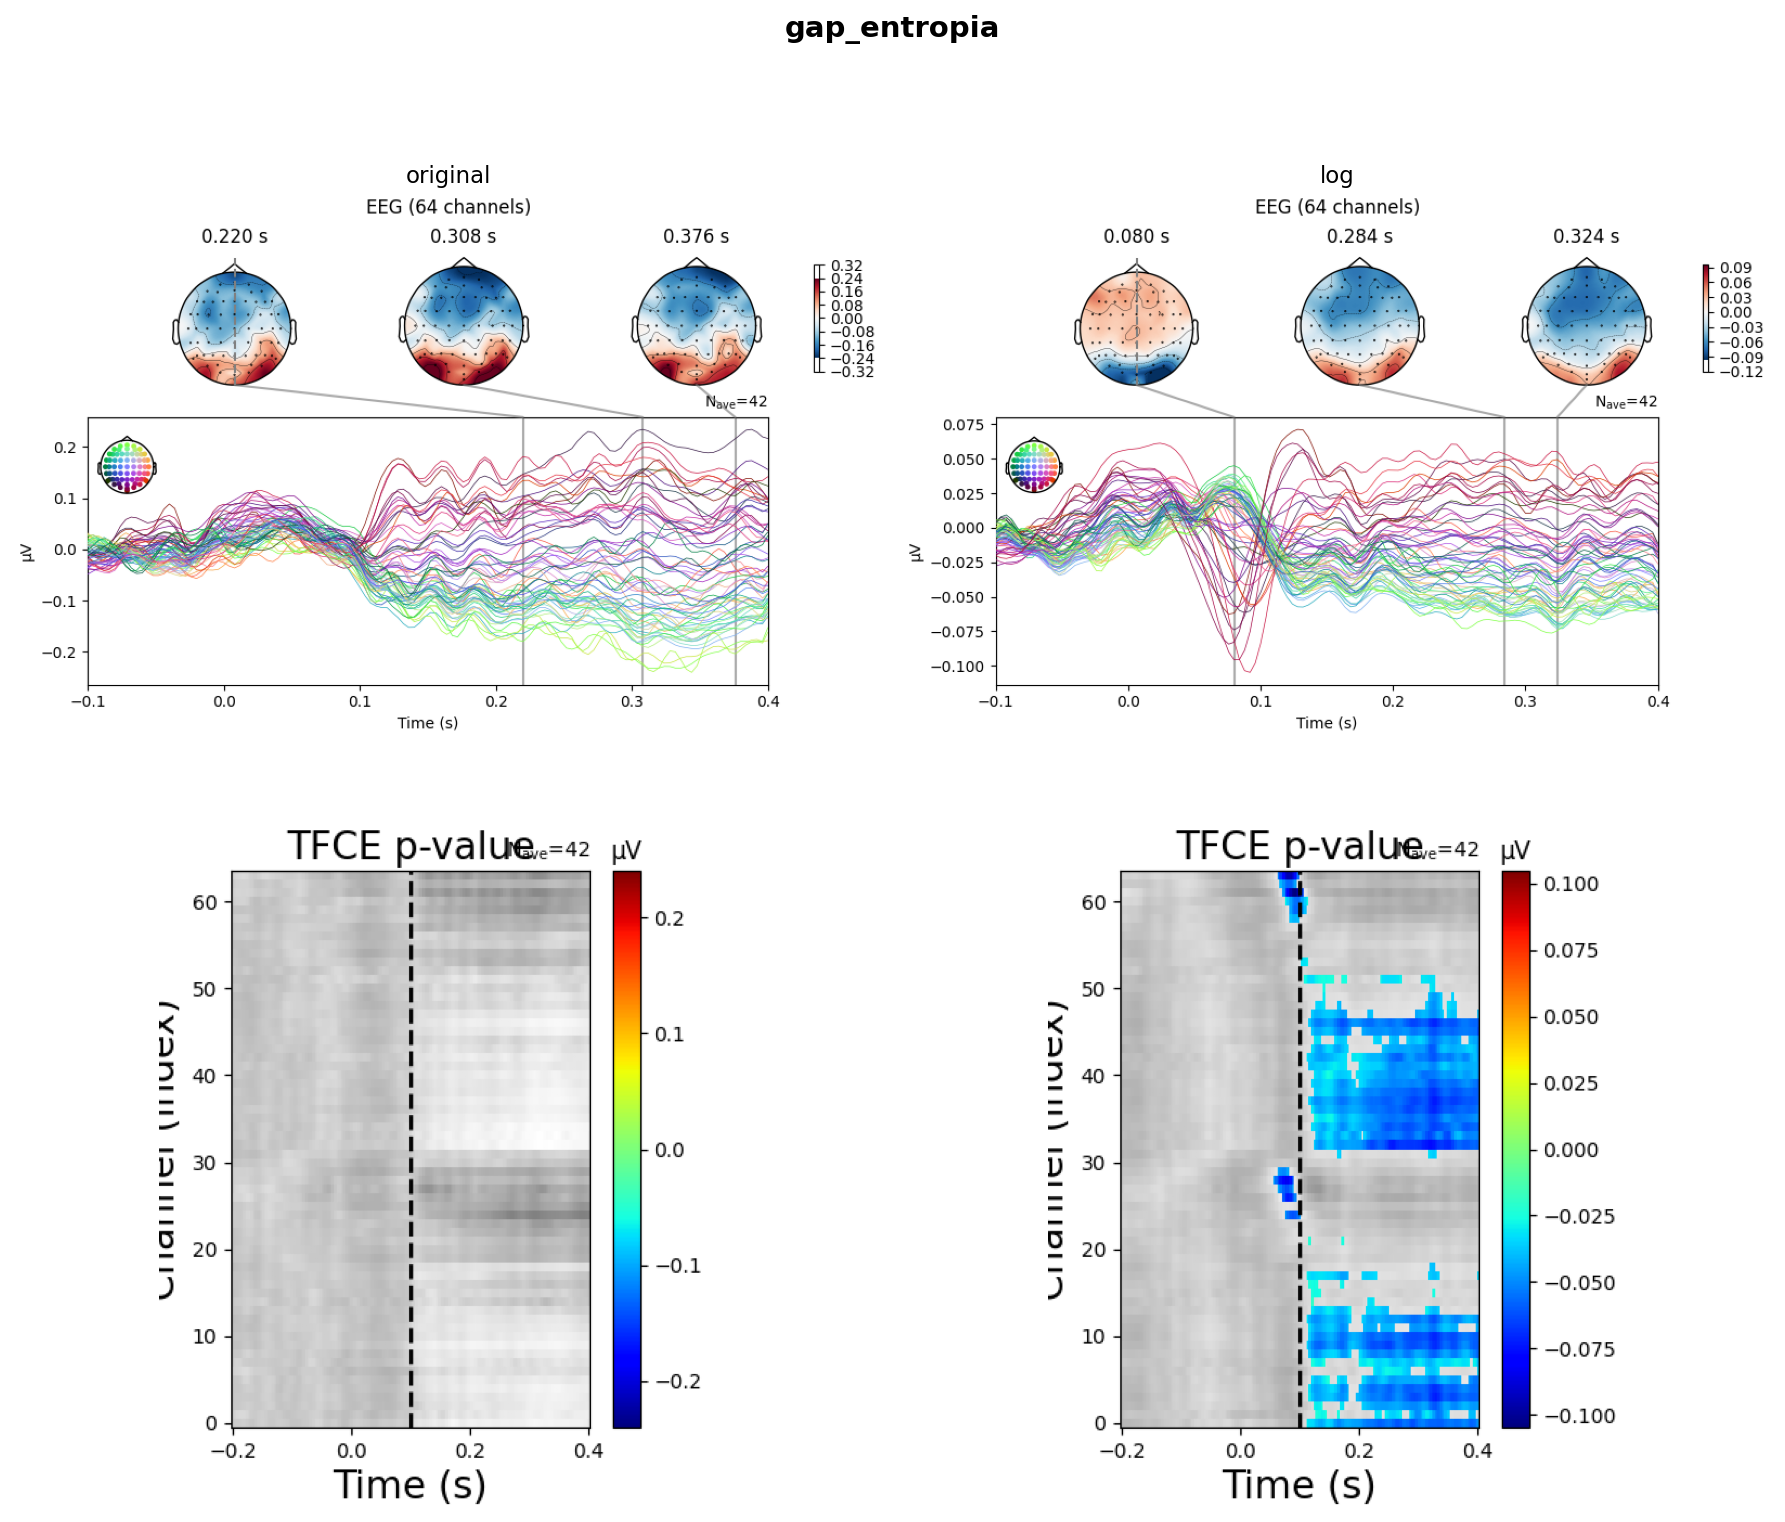
\includegraphics[width=0.7\textwidth]{chapters/05_resultados/images/TFCE_gap_entropia.png}
    \caption{Comparación resultados de TFCE para \feat{gap\_entropia} original y transformada en escala logarítmica.}
    \label{fig:tfce_gap_entropia}
\end{figure}

\subsubsection{Variables sin clusters significativos en ninguna versión}

\feat{competencia\_fp\_max} y \feat{competencia\_fp\_max\_log} no 
presentaron clusters espacio-temporales significativos según el criterio 
TFCE en ninguna de las dos versiones. Este resultado es consistente 
con los valores moderados de $\Delta$AIC observados para ambas versiones: si bien la transformación 
logarítmica mejora el ajuste del modelo respecto al baseline, esta 
mejora no se traduce en efectos estadísticamente significativos a nivel 
espacio-temporal.

\begin{figure}[H]
    \centering
    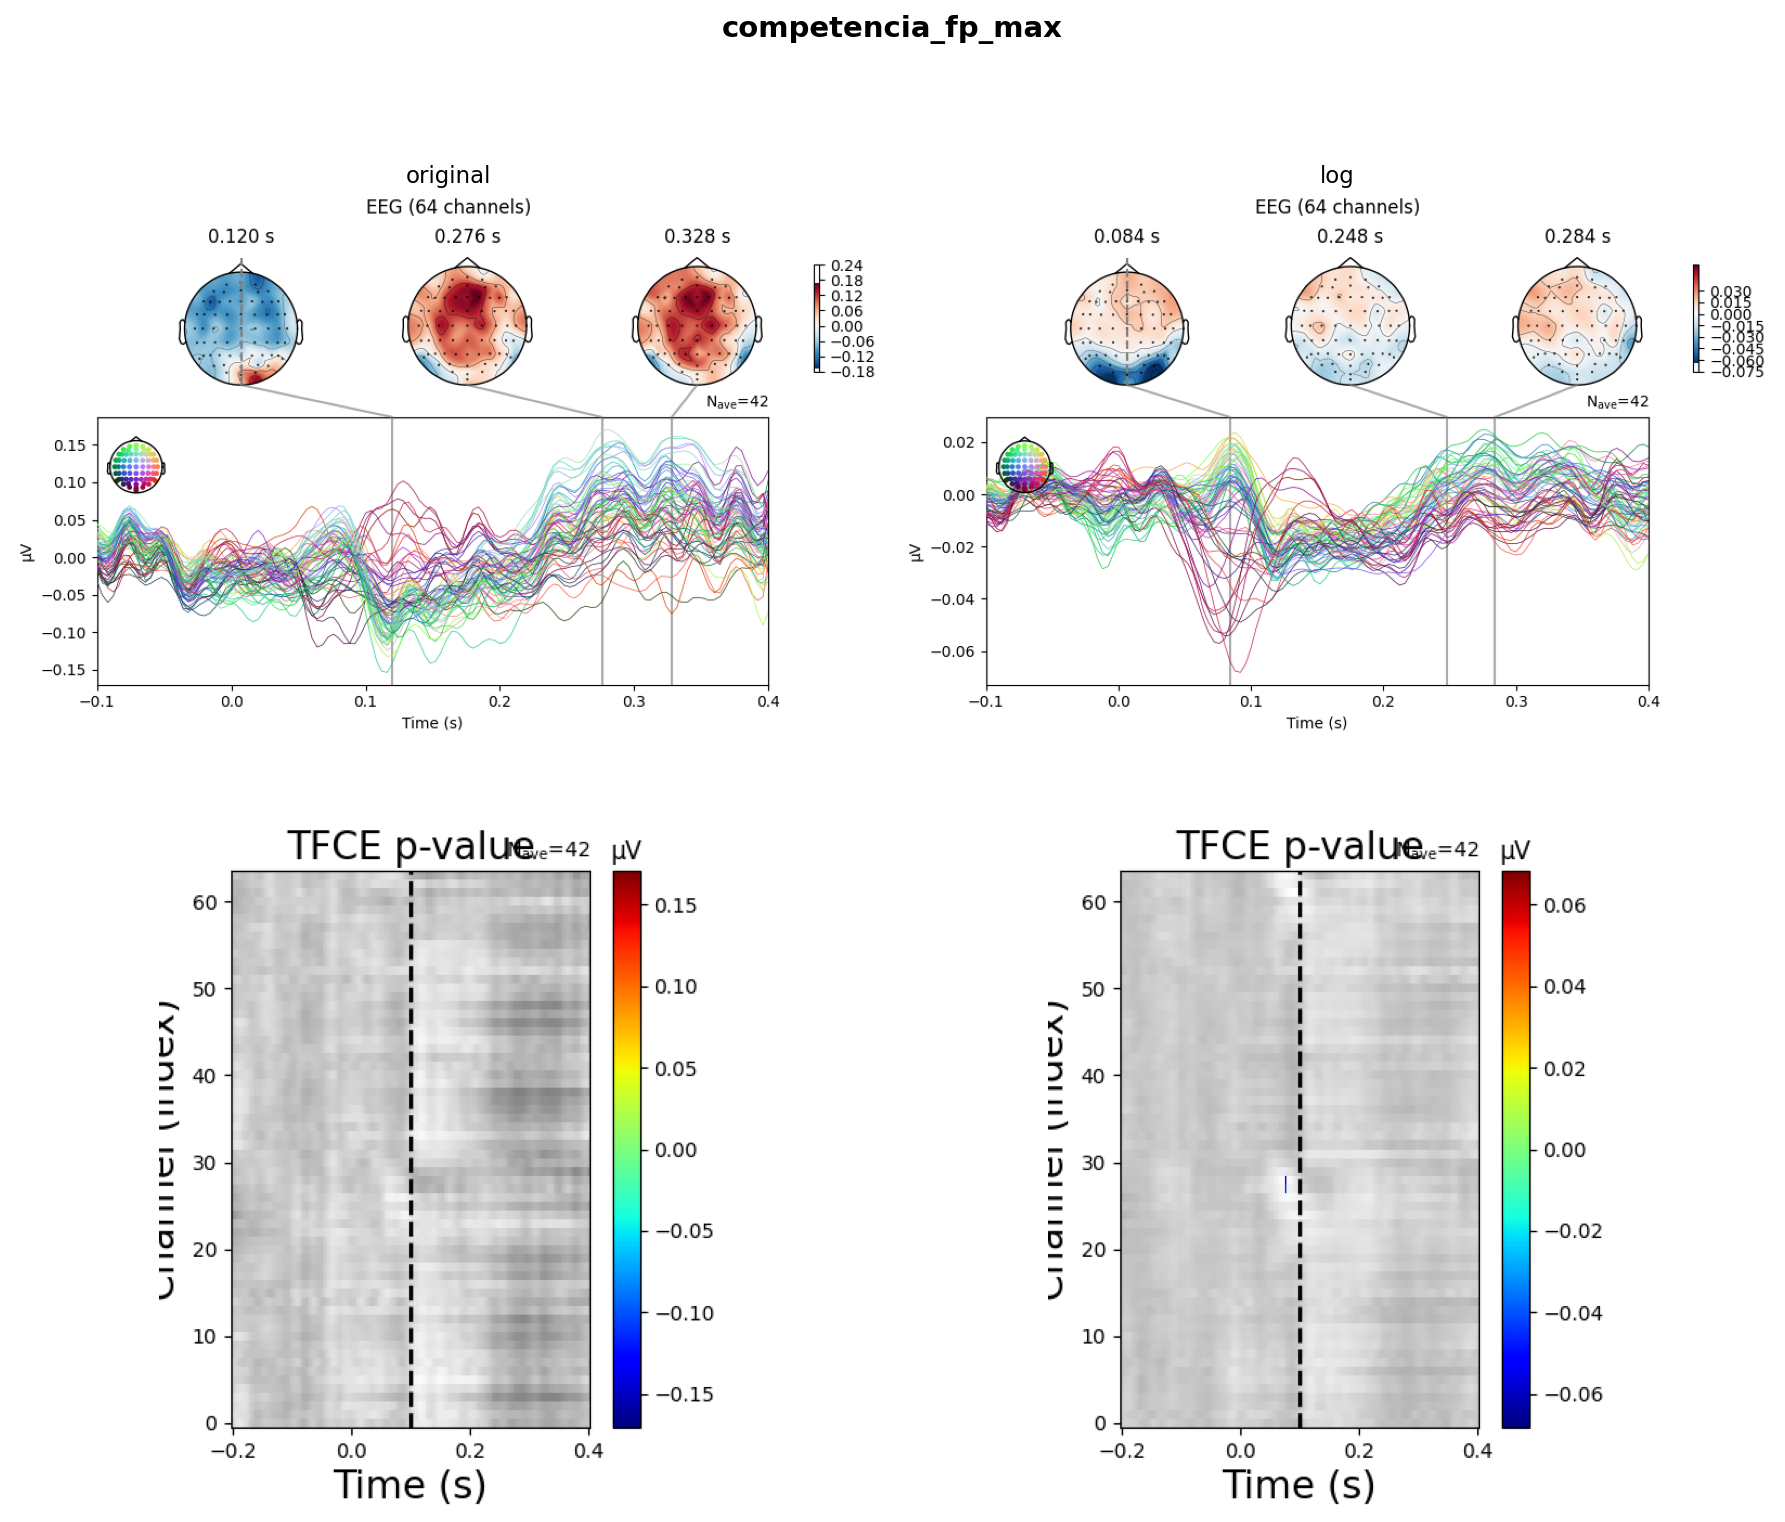
\includegraphics[width=0.7\textwidth]{chapters/05_resultados/images/TFCE_competencia_fp_max.png}
    \caption{Comparación resultados de TFCE para \feat{competencia\_fp\_max} original y transformada en escala logarítmica.}
    \label{fig:tfce_competencia_fp_max}
\end{figure}
